\section{Linux Automations} % Seções são adicionadas para organizar sua apresentação em blocos discretos, todas as seções e subseções são automaticamente exibidas no índice como uma visão geral da apresentação, mas NÃO são exibidas como slides separados.

%----------------------------------------------------------------------------------------


\begin{frame}
  \frametitle{Linux Automations}

Objetivo: remover o overhead cognitivo (não é só executar as tarefas mais rápidas, mas reduzir o esforço mental necessário para gerenciar tarefas repetitivas).
Uma validação: você nao pensa mais em como precisa fazer algo, mas só no que precisa ser feito.
Uma validação além (script -> IA?): quando suas automações te surpreendem, ela já fez algo que você nem lembrava que tinha programado.
Exemplo: acoes programadas no GitHub Actions com base no codigo commitado. Por exemplo, se um arquivo dessa pasta foi alterado entao refaz tal e tal acao, com consequencias bem distantes do codigo original (ex: atualizar um arquivo de log, ou enviar um email, ou criar um pull request, ou atualizar uma planilha, etc).

script vs IA!!!!
Lugares com modelos gratuitos: Hugging Face, OpenAI, etc.

Treinar IAs pros seus próprios objetivos. 
( Construir e treinar modelos de IA personalizados para tarefas específicas, como organização de arquivos, gerenciamento de tarefas, ou até mesmo para responder a perguntas frequentes relacionadas ao seu trabalho. Isso pode ser feito usando plataformas de IA que permitem a criação de modelos personalizados, como o OpenAI GPT-3 ou outras ferramentas de aprendizado de máquina. )

registro de chave criptrográfica para login sem senha
sincronização de arquivos entre máquinas com web socket
sincronização de arquivos entre máquinas com rsync (comandos up down)
./bashrc para configurar terminal 
./bash_profile para configurar ambiente
alias

Comandos para visualizar recursos do sistema: top, htop, free, df, du
Comandos para verificar tarefas sendo executadas no computador



  \centering
  \renewcommand{\arraystretch}{1.15}
\end{frame}



%----------------------------------------------------------------------------------------


% \begin{frame}
%   \frametitle{Tasks Status}

%   \centering
%   \renewcommand{\arraystretch}{1.15}

%   \begin{table}
%     \begin{tabular}{|p{0.58\textwidth}|c|p{0.22\textwidth}|}
%       \hline
%       \textbf{Task} & \textbf{Status} &  \\
%       \hline

%       \textbf{Analisar toy model} &  &  \\
%       \hline

%       \hspace{1.2em}\small$\hookrightarrow$ 
%       & \done &  \\
%       \hline

%       \hspace{1.2em}\small$\hookrightarrow$ 
%       & \done &  \\
%       \hline

%       \hspace{1.2em}\small$\hookrightarrow$ 
%       & \done &  \\
%       \hline

%       \hspace{1.2em}\small$\hookrightarrow$ 
%       & \done &  \\
%       \hline

%       \hspace{1.2em}\small$\hookrightarrow$ 
%       & \inprogress &  \\
%       \hline

%       \hspace{1.2em}\small$\hookrightarrow$ 
%       & \pending &  \\
%       \hline

%     \end{tabular}
%   \end{table}
% \end{frame}

% \begin{frame}
%   \frametitle{Tasks Status}

  % Ajustes úteis em tabelas no Beamer
%   \centering
%   \renewcommand{\arraystretch}{1.15} % mais espaço vertical entre linhas

%   \begin{table}

% \begin{tabular}{|p{0.58\textwidth}|c|p{0.22\textwidth}|}
% \hline
% \textbf{Task} & \textbf{Status} & \textbf{Link} \\
% \hline

% \textbf{Escrever projeto} & &
% \multirow{4}{*}{\centering \href{https://www.overleaf.com/project/696e133a1101ac682ea3dd98}{Projeto}} \\
% \cline{1-2}

% \hspace{1.2em}\small$\hookrightarrow$ Definir escopo e objetivos & \done & \\
% \cline{1-2}

% \hspace{1.2em}\small$\hookrightarrow$ Esboçar introdução (motivação + observáveis) & \done & \\
% \cline{1-2}

% \hspace{1.2em}\small$\hookrightarrow$ Cronograma & \done & \\
% \cline{1-2}

% \hspace{1.2em}\small$\hookrightarrow$ Selecionar bibliografia & \done & \\
% \cline{1-2}

% \hspace{1.2em}\small$\hookrightarrow$ Listar método: GP  & \done & \\
% \cline{1-2}

% \hspace{1.2em}\small$\hookrightarrow$ Listar método: Bayesian Inferente  & \done & \\
% \cline{1-2}

% \hspace{1.2em}\small$\hookrightarrow$ Listar objetivos & \done & \\

% \hline
% \end{tabular}
% \end{table}
% \end{frame}

% \begin{frame}{Uma imagem}
%     \frametitle{Historical Records}
%     In addition, it is possible to retrieve the full search history by running the script directly via GitHub Actions.
%    \begin{figure}[h]
%        \centering
%        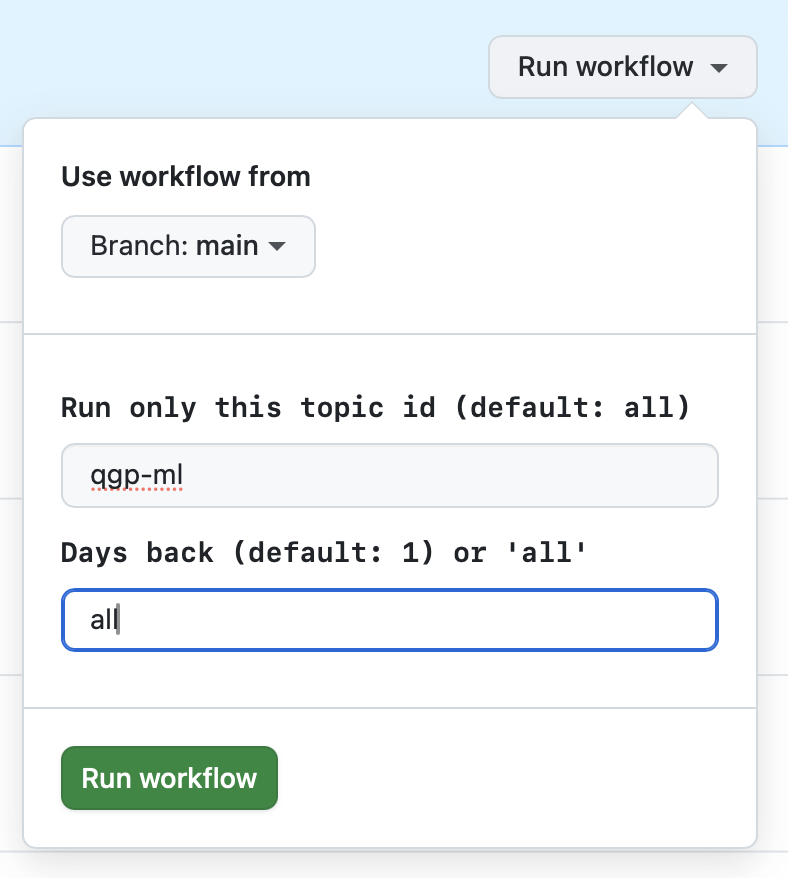
\includegraphics[width=0.3\textwidth]{img/github_topic_history.png}
%        \caption{GitHub Actions interface illustrating how the workflow can be executed to retrieve the full search history for a specific topic.}
%        \label{fig:github_topic_history}
%    \end{figure}
% \end{frame}
%----------------------------------------------------------------------------------------

% \begin{frame}
% 	\frametitle{Texto em tópicos}
%      Lorem ipsum dolor sit amet, consectetur adipiscing elit:
%     \begin{itemize}
%         \item Lorem ipsum dolor sit amet.
%         \item Lorem ipsum dolor sit amet.
%     \end{itemize}
	
% \end{frame}


